\documentclass[compress,t,xcolor=table]{beamer}

%\usepackage[table,xcdraw]{xcolor}

%\input{global.macros}
\usepackage[LGR,T1]{fontenc}

\usepackage{pgf}
\usepackage{pgfplots,pgfplotstable}
\usepackage{tikz}
\usetikzlibrary{shapes,backgrounds}
\usetikzlibrary{arrows,shapes,fit,automata,positioning,decorations,calc}
\usetikzlibrary{spy,backgrounds}
\usepackage{siunitx}
\pgfplotsset{compat=1.12}
\usepackage{tabulary}
\usepackage{multirow}
\usepackage{appendixnumberbeamer}
\usepackage{booktabs}

\usepackage[style=verbose,backend=biber]{biblatex}
\bibliography{references.bib}

\usepackage{listings}
\lstset{language=[LaTeX]TeX,
	numbers=left,
	breaklines=true,
	frame=leftline,
	tabsize=2,
}

\usetheme{Madrid}
\setbeamercovered{transparent}

\definecolor{uoa-blue}{RGB}{3,80,133}
\definecolor{uoa-light-blue}{RGB}{0,154,199}
\definecolor{uoa-grey}{RGB}{230,232,231}

\setbeamercolor{structure}{fg=uoa-blue}

\setbeamertemplate{blocks}[default]
\setbeamercolor{block title}{bg=uoa-blue,fg=white}
\setbeamercolor{block body}{bg=uoa-grey,fg=black}

\setbeamertemplate{title page}[default]

\setbeamertemplate{navigation symbols}{}
%\setbeamertemplate{bibliography item}{\insertbiblabel}

\setbeamertemplate{itemize items}[default]
\setbeamertemplate{enumerate items}[default]

\setbeamertemplate{section in toc}[default]
\setbeamertemplate{subsection in toc}[default]

%\usepackage{fontspec}
%\defaultfontfeatures{Ligatures=TeX}
%\setromanfont{Verdana}

\definecolor{graphFirst}{RGB}{2,136,209} % Light Blue 700
\definecolor{graphSecond}{RGB}{211,47,47} % Red 700
\definecolor{graphThird}{RGB}{245,124,0} % Orange 700
\definecolor{graphFourth}{RGB}{56,142,60} % Green 700
\definecolor{graphFifth}{RGB}{81,45,168} % Deep Purple 700
\definecolor{graphSixth}{RGB}{69,90,100} % Blue Grey 700
\definecolor{graphSeventh}{RGB}{251,192,45} % Yellow 700

\definecolor{backgroundFirst}{RGB}{129,212,250} % Light Blue 200
\definecolor{backgroundSecond}{RGB}{239,154,154} % Red 200
\definecolor{backgroundThird}{RGB}{255,204,128} % Orange 200
\definecolor{backgroundFourth}{RGB}{165,214,167} % Green 200
\definecolor{backgroundFifth}{RGB}{179,157,219} % Deep Purple 200
\definecolor{backgroundSixth}{RGB}{176,190,197} % Blue Grey 200
\definecolor{backgroundSeventh}{RGB}{255,245,157} % Yellow 200

\renewcommand\thefootnote{\textcolor{graphThird}{\arabic{footnote}}}

\newenvironment{myitemize}
{ \begin{itemize}
		\setlength{\itemsep}{10pt}     }
	{ \end{itemize}                  } 


\newenvironment<>{varblock}[2][\textwidth]{%
  \setlength{\textwidth}{#1}
  \begin{actionenv}#3%
    \def\insertblocktitle{#2}%
    \par%
    \usebeamertemplate{block begin}}
  {\par%
    \usebeamertemplate{block end}%
  \end{actionenv}}
  
\AtBeginSection[]
{
	\begin{frame}<beamer>
		\frametitle{Overview}
		\tableofcontents[currentsection]
	\end{frame}
}

\newenvironment{variableblock}[3]{%
	\setbeamercolor{block body}{#2}
	\setbeamercolor{block title}{#3}
	\begin{block}{#1}}{\end{block}}

\usepackage{amsthm}
\setbeamertemplate{theorems}[numbered]

% Keys to support piece-wise uncovering of elements in TikZ pictures:
% \node[visible on=<2->](foo){Foo}
% \node[visible on=<{2,4}>](bar){Bar}   % put braces around comma expressions
%
% Internally works by setting opacity=0 when invisible, which has the 
% adavantage (compared to \node<2->(foo){Foo} that the node is always there, hence
% always consumes space plus that coordinate (foo) is always available.
%
% The actual command that implements the invisibility can be overriden
% by altering the style invisible. For instance \tikzsset{invisible/.style={opacity=0.2}}
% would dim the "invisible" parts. Alternatively, the color might be set to white, if the
% output driver does not support transparencies (e.g., PS) 
%
\tikzset{
	invisible/.style={opacity=0},
	visible on/.style={alt={#1{}{invisible}}},
	alt/.code args={<#1>#2#3}{%
		\alt<#1>{\pgfkeysalso{#2}}{\pgfkeysalso{#3}} % \pgfkeysalso doesn't change the path
	},
}

\tikzset{onslide/.code args={<#1>#2}{%
	\only<#1>{\pgfkeysalso{#2}}
}}
\tikzstyle{highlight}=[red!90, fill=red!5]
\tikzstyle{highlightsource}=[blue!90, fill=blue!5]
\tikzstyle{borderhighlight}=[red!90, text=black, fill=red!5]
\tikzstyle{texthighlight}=[text=red!90, fill=red!5]

\newcommand{\code}[1]{{\small{\texttt{#1}}}}
\newcommand{\todo}[1]{{\color{orange}(TODO: #1)}}

\title[Keyan Monadjem Master's Project]{Synchronous Artificial Neural Networks for Safety Critical Systems}

\author[]{\large Keyan Monadjem}

\institute[University of Auckland]
{
	
\includegraphics[scale=0.3]{fig/UOA-HC-RGB.png}
}

\date[]{
	August 17, 2018
}

\begin{document}

%%%%%%%%%%%%%%%%%%%%%%%%%%%%%%%%%%%%%%%%%%%%%%%%%%%%%%%%%%%%%%%%%%%%%%
\frame{\titlepage}


%%%%%%%%%%%%%%%%%%%%%%%%%%%%%%%%%%%%%%%%%%%%%%%%%%%%%%%%%%%%%%%%%%%%%%
\section{Introduction}

\begin{frame} \frametitle{What is Artificial Intelligence?}
	The aim for machines to intelligently decide the best course of action to meet their respective goals.
	\begin{block}{Machine-based...}
		\begin{myitemize}
			\item Acquisition and Manipulation of Knowledge
			\item Generation and Achievement of Goals
		\end{myitemize}
	\end{block}
\end{frame}

\begin{frame} \frametitle{Are they useful?}
	\centering
	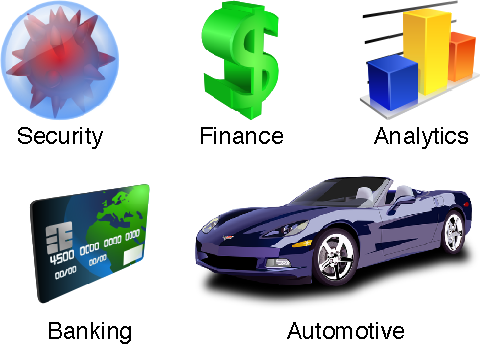
\includegraphics[scale=0.9]{fig/AI-uses.pdf}
	
	\vspace{10mm}
	
	\emph{Image/Pattern Recognition}
\end{frame}

\begin{frame} \frametitle{There are many kinds of AI}
	\begin{block}{(Some) Types}
		\begin{myitemize}
			\item Symbolic AI
			\item Statistical Learning
			\item Sub-symbolic	\begin{myitemize}
				\item Evolutionary Computation
				\item Probabilistic Modelling
				\item \textbf{Artificial Neural Networks (ANNs)}
			\end{myitemize}
		\end{myitemize}
	\end{block}
\end{frame}

\begin{frame} \frametitle{AI is \textit{reactive}...}
	\centering
	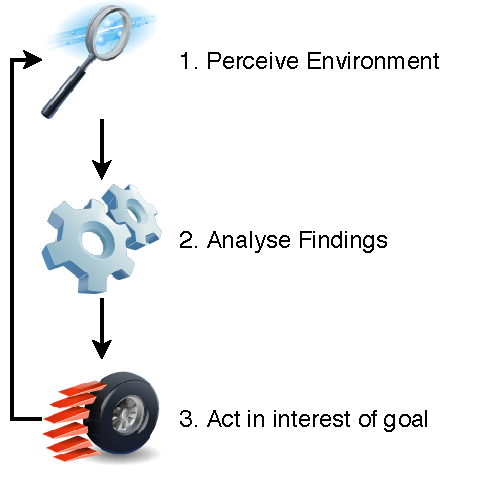
\includegraphics[scale=0.9]{fig/reactive-AI.pdf}
\end{frame}


\begin{frame} \frametitle{Reactive Safety-Critical Systems}
	\centering
	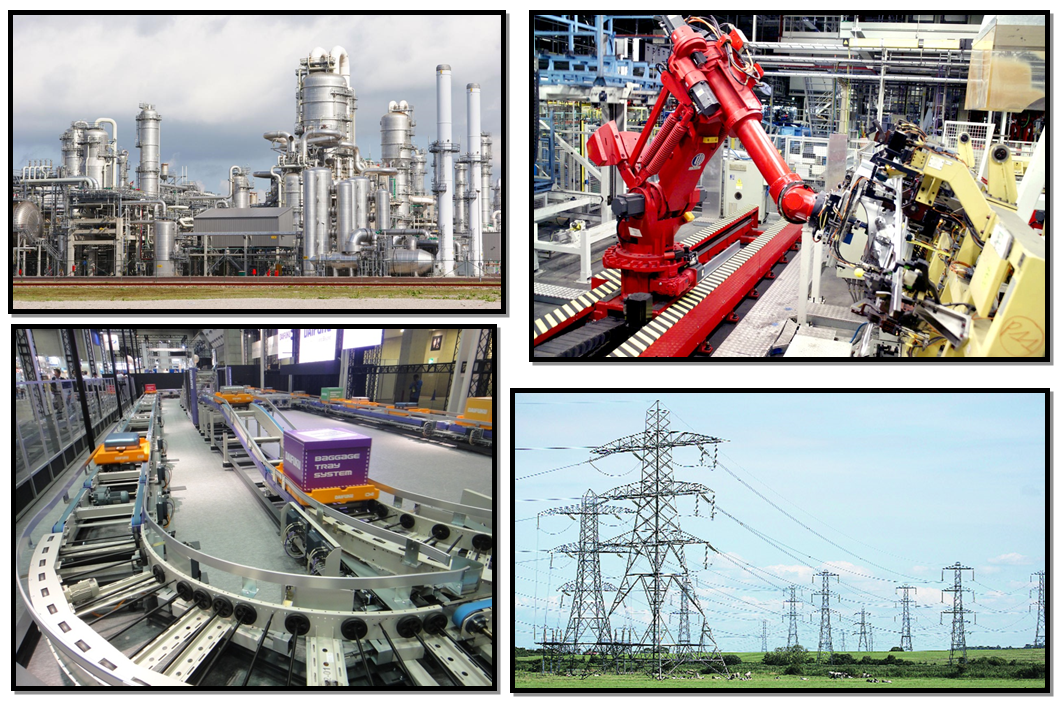
\includegraphics[scale=0.4]{fig/1234.png}
\end{frame}

%\begin{frame} \frametitle{AI Controllers?}
%	\centering
%	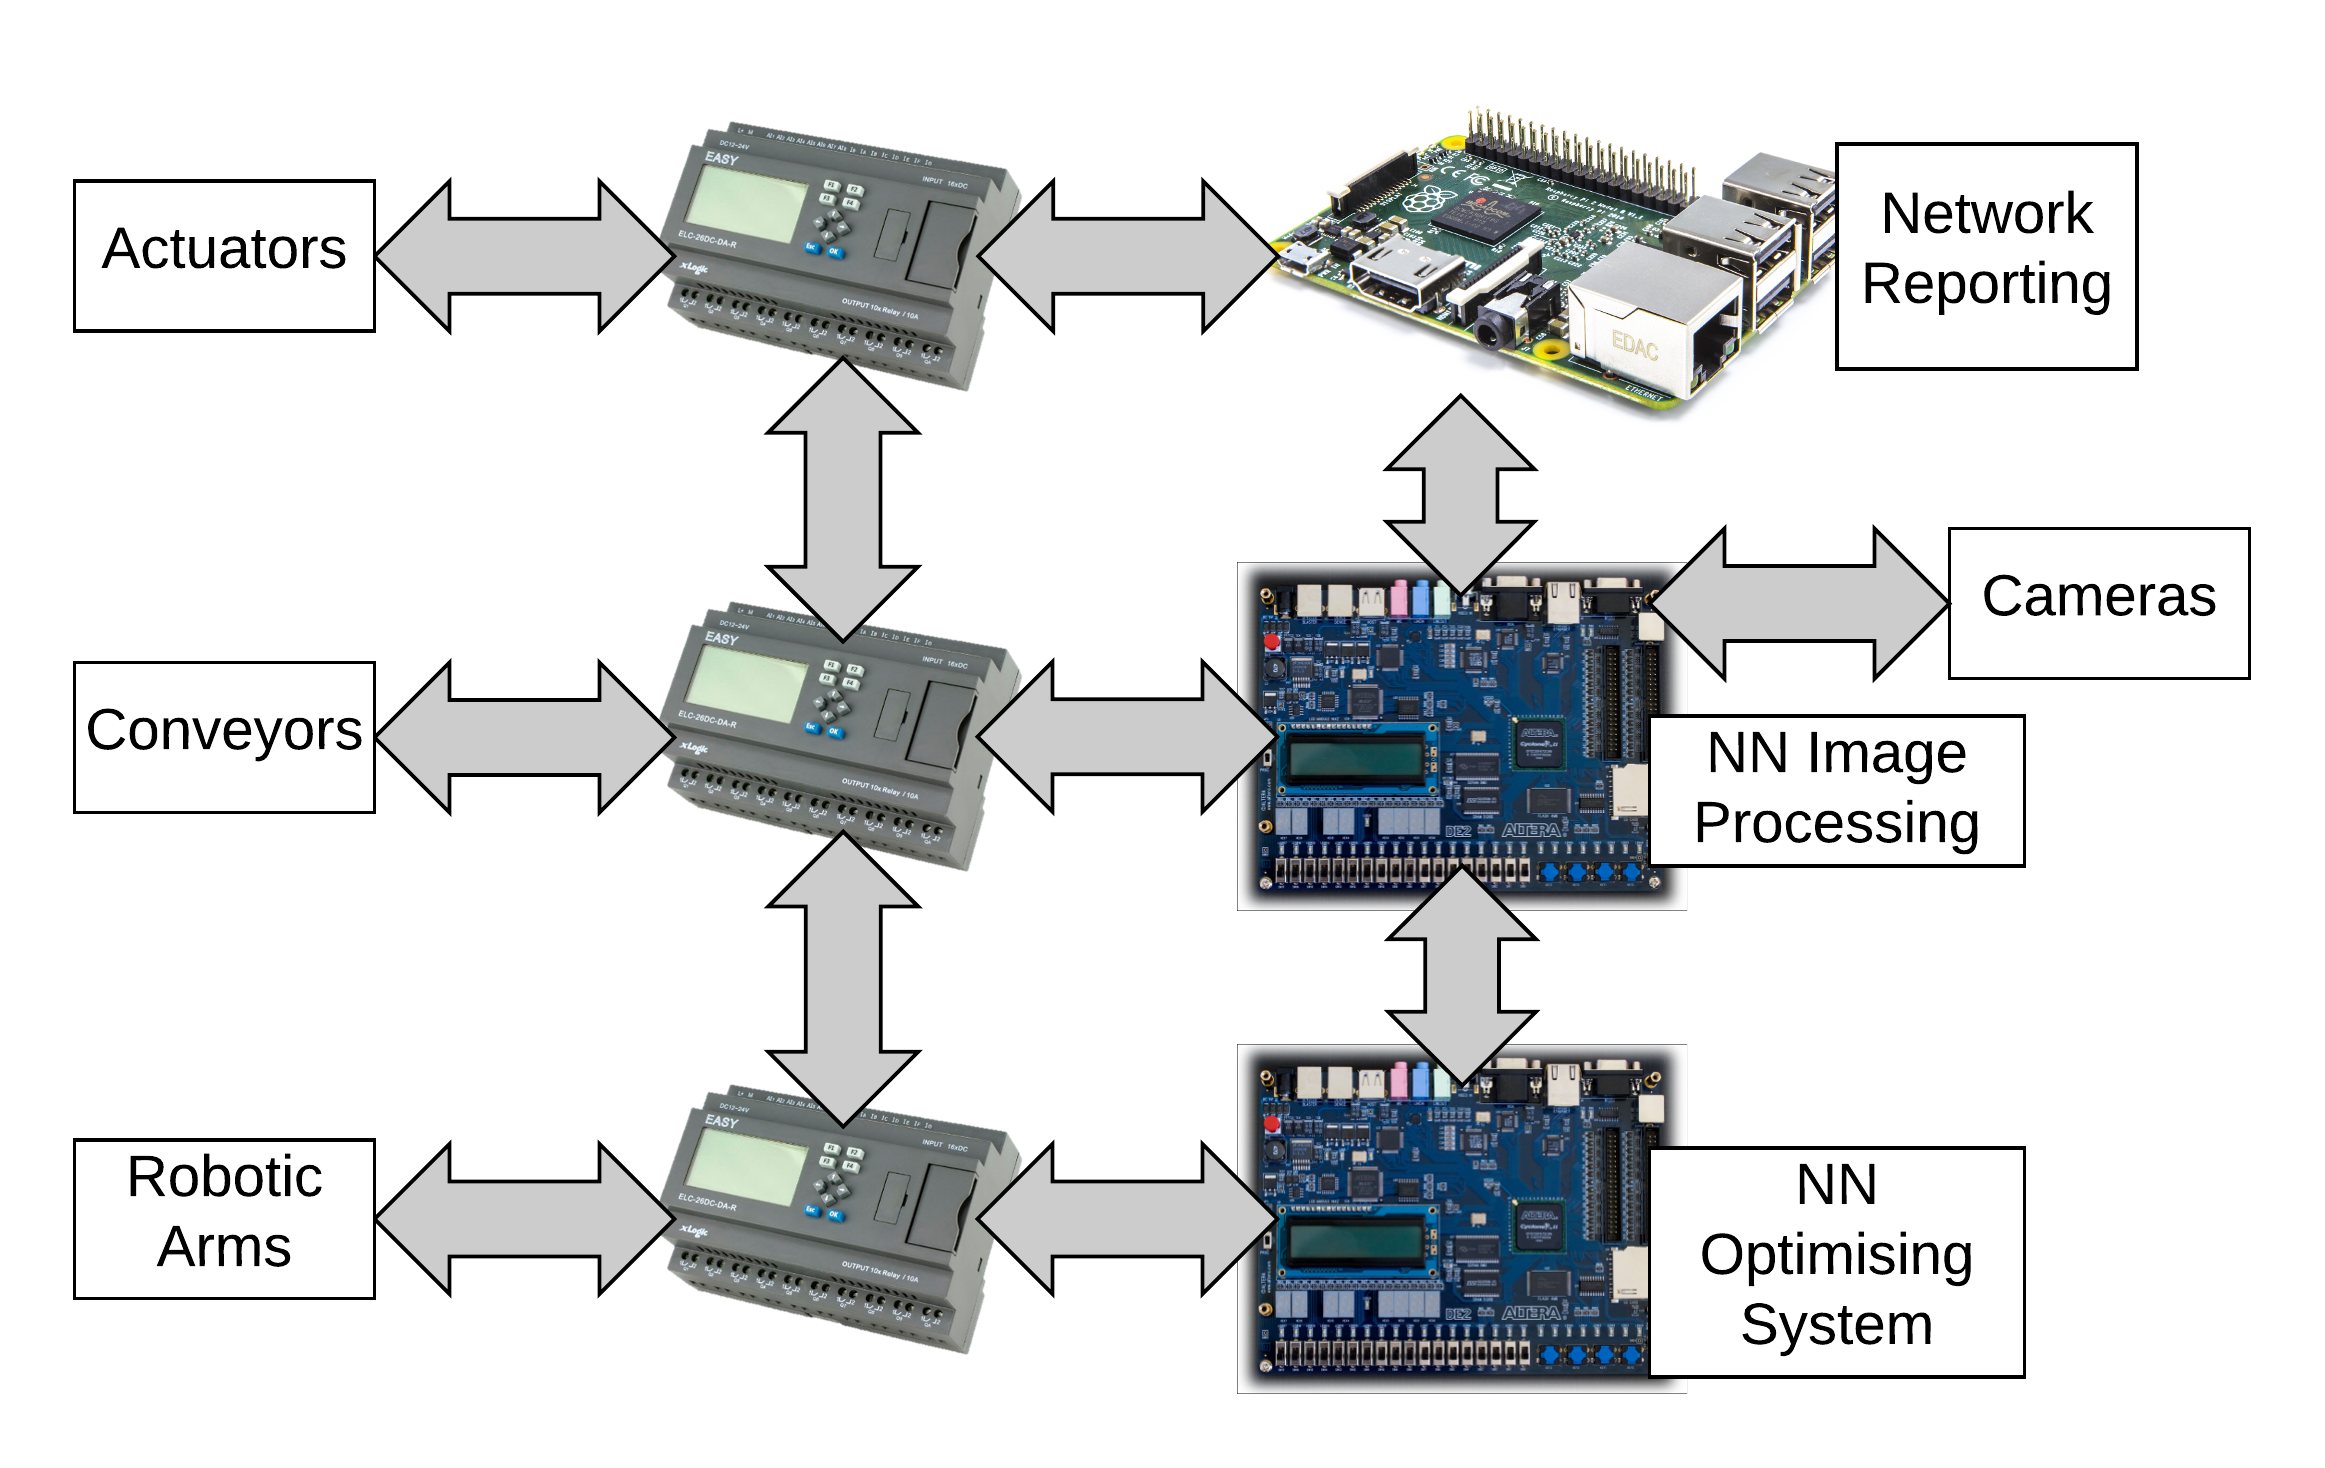
\includegraphics[scale=0.6]{fig/ad-hoc-network.png}
%\end{frame}

\section{Background}

\begin{frame} \frametitle{A brief overview of ML}
	Software that learns data relationships without the software knowing the relationships beforehand.
	\begin{block}
		\centering
		\begin{myitemize}
			\item Decision trees
			\item \textbf{ANNs - deep learning}
			\item Reinforcement learning
		\end{myitemize}
	\end{block}
\end{frame}

\begin{frame} \frametitle{A brief overview of ANNs}
	\begin{myitemize}
		\item Originally designed to model the brain.
		\item One neural network is a group of interconnected nodes, called artificial neurons, which pass signals among themselves.
	\end{myitemize}
	\begin{columns}
		\begin{column}{0.45\linewidth}	
			\begin{figure}[t]
				\centering
				\scalebox{0.5}{\def\layersep{2.25cm}
\def\numInp{4}
\def\numHid{5}
\def\numOut{3}
\begin{tikzpicture}[shorten >=1pt,->,draw=black!100, node distance=\layersep]
	\tikzstyle{every pin edge}=[<-,shorten <=1pt]
	\tikzstyle{neuron}=[circle,fill=black!25,minimum size=20pt,inner sep=0pt]
	\tikzstyle{input neuron}=[neuron, fill=white!100,draw=black];
	\tikzstyle{output neuron}=[neuron, fill=white!100,draw=black];
	\tikzstyle{hidden neuron}=[neuron, fill=white!100,draw=black];
	\tikzstyle{annot} = [text width=4em, text centered]
	
	% Draw the input layer nodes
	\foreach \name / \y in {1,...,\numInp}
	% This is the same as writing \foreach \name / \y in {1/1,2/2,3/3,4/4}
	\node[input neuron, pin=left:Input \y] (I-\name) at (0,-\y) {$i_\y$};
	
	% Draw the hidden layer nodes
	\foreach \name / \y in {1,...,\numHid}
	\path[yshift=0.5cm]
	node[hidden neuron] (H-\name) at (\layersep,-\y cm) {$h_\y$};
	
	% Draw the output layer nodes
	\foreach \name / \y in {1,...,\numOut}
	\node[output neuron, pin={[pin edge={->}]right:Output \y}] (O-\name) at (4.5,-0.25-\y) {$o_\y$};
		
	% Connect every node in the input layer with every node in the
	% hidden layer.
	\foreach \source in {1,...,\numInp}
	\foreach \dest in {1,...,\numHid}
	\path (I-\source) edge (H-\dest);
	
	% Connect every node in the hidden layer with the output layer
	\foreach \source in {1,...,\numHid}
	\foreach \dest in {1,...,\numOut}
	\path (H-\source) edge (O-\dest);
	
	% Annotate the layers
	\node[annot,above of=H-1, node distance=1cm] (hl) {\textit{Hidden Layer}};
	\node[annot,left of=hl] {\textit{Input Layer}};
	\node[annot,right of=hl] {\textit{Output Layer}};
\end{tikzpicture}}
				\caption{Example of an ANN.	\label{fig:ann}}
			\end{figure}
		\end{column}
		\begin{column}{0.45\linewidth}
			\begin{figure}[t]
				\centering
				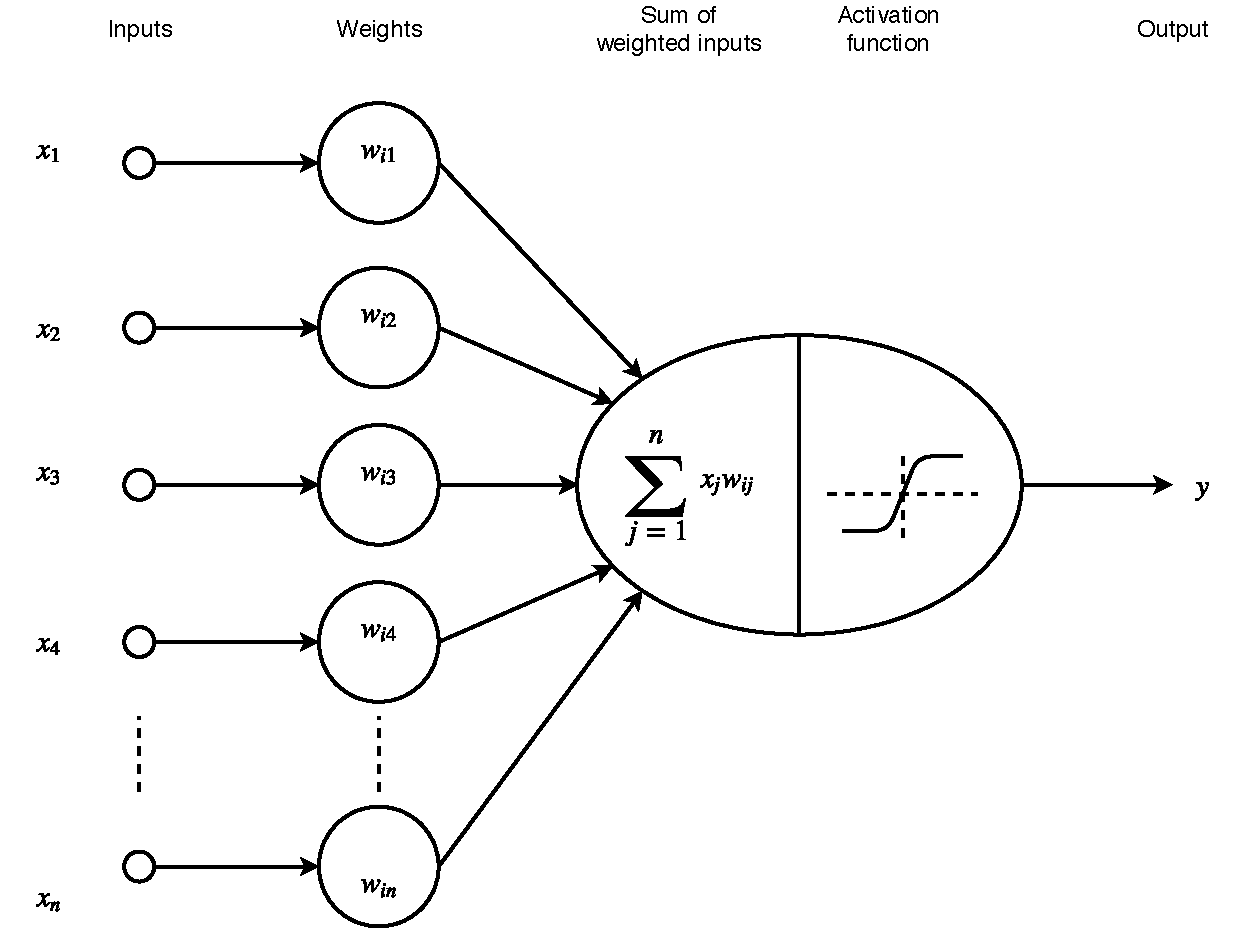
\includegraphics[scale=0.2]{fig/ArtificialNeuron.pdf}
				\caption{Example of an artificial neuron.	\label{fig:neuron}}
			\end{figure}
		\end{column}
	\end{columns}
\end{frame}

\begin{frame} \frametitle{Verified ANNs for safety critical systems}
	\begin{myitemize}
		\item Software/systems based on ML can be very complex.
		\item Not suitable for safety critical systems without validation/verification.
		\item Existing techniques to verify/validate ANNs for safety critical environments (proactive) - not always ideal.
		\item Few solutions for \textit{reactive} safety critical ANNs.
		\item Functional Analysis and formal methods (e.g. \textbf{WCRT}).
		\item \textbf{Runtime Enforcement}.
	\end{myitemize}
\end{frame}

\section{Existing Solutions for Safety-Critical AI Systems}

\begin{frame} \frametitle{Current AI in safety-critical applications}
	\begin{block}{Validation and Verification}
		\begin{myitemize}
			\item Unit testing
			\item Strict guidelines~\nocite{ANNDevModel1999}
			\item Verification algorithms~\footcite{safe_verify}\footcite{reluplex}\footcite{ai2} 
		\end{myitemize}
	\end{block}
\end{frame}

\begin{frame}
	\begin{block}{Safety Critical Artificial Neural Networks (SCANNs) \footcite{scann}}
		\begin{myitemize}
			\item Fuzzy Self-Organising Maps (FSOMs)
			\item Rule extraction and insertion
			\item Safety cases
		\end{myitemize}
	\end{block}
\end{frame}

\begin{frame} \frametitle{Why Are Current Implementations \textit{Bad}?}
	\begin{myitemize}
		\item Difficult to formally quantify an ANN.
		\item Verification of ANNs hot topic and highly researched.
		\item Does not address faulty run-time outputs.
	\end{myitemize} 
\end{frame}

\section{Motivating example}
\begin{frame} \frametitle{Uber autonomous vehicle fatal accident} 
	\begin{block}{What happened?}\footcite{uber1}
		\begin{myitemize}
			\item Uber autonomous vehicle.
			\item Vehicle collided with jaywalking pedestrian.
			\item \textbf{Fatal}.
		\end{myitemize}
	\end{block}
\end{frame}
\begin{frame}
	\begin{block}{What went wrong?}
		\begin{myitemize}
			\item Pedestrian was sufficiently inebriated.
			\item ANN misclassified the pedestrian \textbf{multiple times}.
			\item Software (AI) trusted over LiDAR readings.
			\item Vehicle did not brake and driver was not paying attention.
			\item Failure on many fronts, including the software of a \textit{safety critical} system.
		\end{myitemize}
	\end{block}
\end{frame}
\begin{frame}\frametitle{Problem Statement}
	How can artificial neural networks utilise synchronous languages such that the safety and performance of safety-critical systems is improved?
\end{frame}

\section{Solution: Utilising Synchronous Semantics}

\begin{frame} \frametitle{Introduction to Synchronous Semantics~\footcite{benveniste2003synchronous}}
	\begin{myitemize}
		\item No chance of deadlocks occurring during runtime.
		\item Loops are bounded.
		\item Causality is maintained.
		\item System is deterministic.
		\item Runtime enforcement and observers.
		\item Easier to formally analyse Worst Case Execution Time (WCET) and Worst Case Reaction Time (WCRT).
	\end{myitemize}
\end{frame}

\begin{frame} \frametitle{WCET}
	\begin{myitemize}
		\item Blackbox ANN that "runs fast enough" - not good enough.
		\item WCET of ANNs using formal methods largely unexplored.
		\item WCET analysis is usually measurement-based .
	\end{myitemize}
\end{frame}

\begin{frame} \frametitle{Synchronous Artificial Neural Networks (SANNs)}
	\begin{myitemize}
		\item Created upon the basis of synchronous semantics using Esterel.
		\item Receives all the bonuses of a synchronous language.
		\item Various ANN compositions, both inter-network (meta neural networks) and intra-network (network scheduling).
	\end{myitemize}
	\begin{columns}
		\begin{column}{0.45\textwidth}
			\begin{figure}[h]
				\centering
				\scalebox{0.8}{\begin{tikzpicture}[->,>=stealth',shorten >=1pt,auto,
node distance=2.5cm,
semithick,scale=0.8, transform shape,scale=0.6, font=\huge]

\tikzstyle{every state}=[ellipse, minimum width=2cm, minimum height=1.5cm, text centered, 
fill=blue!20,draw=none,text=black, draw,line width=0.3mm, font=\LARGE]

%start state
\node[state]
(init) 
{$l_i \odot l_h \odot l_o$}; 

\draw[->] (init.south) 
|- ($(init.south) + (0, -0.75cm)$) 
-| ($(init.east) + (0.25cm, 0)$) 
|- ($(init.east) + (0, 1.5cm)$) 
-| (init.north);

\end{tikzpicture}
}
				\caption{Black box execution of an SANN.	\label{fig:sann-bb}}
			\end{figure}
		\end{column}
		%\begin{column}{0.45\textwidth}
		%	\begin{figure}[h]
		%		\begin{lstlisting}[caption={Esterel implementation of black box scheduling},label={lst:bb}]
		%		loop
		%			call run_ANN_i()(?x1, ?x2);
		%			call run_ANN_h()();
		%			emit y(run_ANN_o()());
		%			pause;
		%		pause;
		%		end
		%		\end{lstlisting}
		%	\end{figure}
		%\end{column}
	\end{columns}
\end{frame}

\begin{frame} \frametitle{Black-box scheduling}
	\begin{myitemize}
		\item Single function call to run the entire neural network in one synchronous tick.
		\item Inputs are provided, outputs are returned.
	\end{myitemize}
	\begin{block}{Disadvantages}
		\begin{myitemize}
			\item Function calls from synchronous programs are hardly new.
			\item Iterates through all layers of the Neural Network in one tick - slow.
			\item High WCRT should the system fail.
		\end{myitemize}
	\end{block}
\end{frame}

\begin{frame} \frametitle{Layer by Layer scheduling}
	\begin{myitemize}
		\item Each synchronous tick runs one layer of the neural network
		\item Between layer results are stored to be used in the next tick
		\item Faster WCRT than black box - system can respond between layers
	\end{myitemize}
	\begin{columns}
		\begin{column}{0.45\textwidth}
			\begin{figure}[h]
				\centering
				\scalebox{0.8}{\begin{tikzpicture}[->,>=stealth',shorten >=1pt,auto,
node distance=2.5cm,
semithick,scale=0.8, transform shape,scale=0.6, font=\huge]

\tikzstyle{every state}=[ellipse, minimum width=2.5cm, minimum height=1.5cm, text centered, 
fill=blue!20,draw=none,text=black, draw,line width=0.3mm, font=\LARGE]

%start state
\node[state]
(l0) 
{$l_i$};

\node[state]
(l1) [below of=l0]
{$l_h$}; 

\node[state]
(l2) [below of=l1]
{$l_o$};  

\path[->] (l0) edge (l1);
\path[->] (l1) edge (l2);

\draw[->] (l2.south) 
|- ($(l2.south) + (0, -0.75cm)$) 
-| ($(l2.east) + (1cm, 0)$) 
|- ($(init.east) + (0, 1.5cm)$) 
-| (init.north);

\end{tikzpicture}
}
				\caption{Layer by layer execution of an SANN.	\label{fig:sann-l}}
			\end{figure}
		\end{column}
		%\begin{column}{0.45\textwidth}
		%	\begin{figure}[h]
		%		\begin{lstlisting}[caption={Esterel implementation of layer by layer scheduling},label={lst:l}]
		%		loop
		%			call run_ANN_i()(?x1, ?x2);
		%			pause;
		%			call run_ANN_h()();
		%			pause;
		%			emit y(run_ANN_o()());
		%			pause;
		%		end
		%		\end{lstlisting}
		%	\end{figure}
		%\end{column}
	\end{columns}
\end{frame}

\begin{frame} \frametitle{Neuron by Neuron scheduling}
	\begin{myitemize}
		\item Each artificial neuron created in Esterel.
		\item Each synchronous tick runs one layer of the neural network.
		\item Each layer connected by signals to previous and/or following layers.
		\item Faster WCRT than layer by layer scheduling - less overhead.
	\end{myitemize}
	\begin{columns}
		\begin{column}{0.45\textwidth}
			\begin{figure}[h]
				\centering
				\scalebox{0.8}{\begin{tikzpicture}[->,>=stealth',shorten >=1pt,auto,
node distance=2.5cm,
semithick,scale=0.8, transform shape,scale=0.6, font=\huge]

\tikzstyle{every state}=[ellipse, minimum width=2.5cm, minimum height=1.5cm, text centered, 
fill=blue!20,draw=none,text=black, draw,line width=0.3mm, font=\LARGE]

%start state
\node[state]
(l0) 
{$i_1 \odot i_2$};

\node[state]
(l1) [below of=l0]
{$h_1 \odot h_2 \odot h_3$}; 

\node[state]
(l2) [below of=l1]
{$o_1$};  

\path[->] (l0) edge (l1);
\path[->] (l1) edge (l2);

\draw[->] (l2.south) 
|- ($(l2.south) + (0, -0.75cm)$) 
-| ($(l2.east) + (1cm, 0)$) 
|- ($(init.east) + (0, 1.5cm)$) 
-| (init.north);

\end{tikzpicture}
}
				\caption{Neuron by neuron execution of an SANN.	\label{fig:sann-n}}
			\end{figure}
		\end{column}
		%\begin{column}{0.45\textwidth}
		%	\begin{figure}[h]
		%	\begin{lstlisting}[caption={Esterel implementation of neuron by neuron scheduling},label={lst:n}]
		%		loop
		%			[
		%				call run_ANN_i1()(?x1);
		%				||
		%				call run_ANN_i2()(?x2);
		%			];
		%			pause;
		%			[
		%				call run_ANN_h1()();
		%				||
		%				call run_ANN_h2()();
		%				||
		%				call run_ANN_h3()();
		%			];
		%			pause;
		%				emit y(run_ANN_o1()());
		%			pause;
		%		end
		%	\end{lstlisting}
		%	\end{figure}
		%\end{column}
	\end{columns}
\end{frame}

\begin{frame} \frametitle{Meta Neural Networks}
	\begin{myitemize}
		\item A composition of SANN black boxes or otherwise.
		\item Intricate combinations feasible due to synchronous semantics.
	\end{myitemize}
	\begin{columns}
		\begin{column}{0.45\linewidth}	
			\begin{figure}[t]
				\centering
				\scalebox{0.8}{\begin{tikzpicture}[->,>=stealth',shorten >=1pt,auto,
node distance=3cm,
semithick,scale=0.8, transform shape,scale=0.6, font=\LARGE]

\tikzstyle{every state}=[rectangle, minimum width=2cm, minimum height=1.5cm, text centered, 
fill=blue!20,draw=none,text=black, draw,line width=0.3mm, font=\LARGE]

\tikzstyle{every ellips}=[fill=none,text=black,line=none,font=\LARGE]

%start state
\node[state]
(n1)
{$M_1$}; 

\node[state]
(n2) [below of=n1]
{$M_2$};

\node[state]
(n3) [right of=n1]
{$M_3$};

\node[state]
(n4) [right of=n2]
{$M_4$}; 

\node[state]
(n5) [right of=n3]
{$M_5$};

\node[state]
(n6) [right of=n4]
{$M_6$}; 

\node[state,fill=none, draw=none]
(el1) [right of=n5]
{...};

\node[state,fill=none, draw=none]
(el2) [right of=n6]
{...};

\node[state]
(nn) [right of=el1]
{$M_n$};

\node[state]
(nn1) [right of=el2]
{$M_{n+1}$};

\path[->] (n1) edge (n3);
\path[->] (n1) edge (n4);
\path[->] (n2) edge (n3);
\path[->] (n2) edge (n4);
\path[->] (n3) edge (n5);
\path[->] (n3) edge (n6);
\path[->] (n4) edge (n5);
\path[->] (n4) edge (n6);
\path[-] (n5) edge (el1);
\path[-] (n5) edge (el2);
\path[-] (n6) edge (el1);
\path[-] (n6) edge (el2);
\path[->] (el1) edge (nn);
\path[->] (el1) edge (nn1);
\path[->] (el2) edge (nn);
\path[->] (el2) edge (nn1);


\end{tikzpicture}
}
				\caption{Example meta neural network with parallel SANNs.	\label{fig:meta-complex2}}
			\end{figure}
		\end{column}
		\begin{column}{0.45\linewidth}
			
			\begin{figure}[t]
				\centering
				\scalebox{0.8}{\begin{tikzpicture}[->,>=stealth',shorten >=1pt,auto,
node distance=3cm,
semithick,scale=0.8, transform shape,scale=0.6, font=\LARGE]

\tikzstyle{every state}=[rectangle, minimum width=2cm, minimum height=1.5cm, text centered, 
fill=blue!20,draw=none,text=black, draw,line width=0.3mm, font=\LARGE]

\tikzstyle{every ellips}=[fill=none,text=black,line=none,font=\LARGE]

%start state
\node[state]
(n1)
{$M_1$}; 

\node[state]
(n2) [below of=n1]
{$M_2$};

\node[state]
(n3) [right of=n1, yshift=-1.5cm]
{$M_3$};

\node[state]
(n4) [right of=n3, yshift=1.5cm]
{$M_4$};

\node[state]
(n5) [below of=n4]
{$M_5$};

\node[state]
(n6) [right of=n4, yshift=-1.5cm]
{$M_6$};

\node[state,draw=none,fill=none]
(el1) [right of=n6, yshift=1.5cm]
{...}; 

\node[state,draw=none,fill=none]
(el2) [below of=el1]
{...}; 


\path[->] (n1) edge (n3);
\path[->] (n2) edge (n3);
\path[->] (n3) edge (n4);
\path[->] (n3) edge (n5);
\path[->] (n4) edge (n6);
\path[->] (n5) edge (n6);
\path[->] (n6) edge (el1);
\path[->] (n6) edge (el2);

\end{tikzpicture}
}
				\caption{Example meta neural network with some parallel SANNs.	\label{fig:meta-complex1}}
			\end{figure}
		\end{column}
	\end{columns}
\end{frame}

\begin{frame} \frametitle{Runtime Enforcement~\footcite{SyncRTE2017}}
	\begin{myitemize}
		\item Monitors and corrects a system's I/O.
		\item Cannot delay events or block execution.
		\item E.g. enforce that the vehicle will brake, instead of accelerating, when a collision could occur.
	\end{myitemize}
	\begin{block}{Observers}
		\begin{myitemize}
			\item Statically specify properties of a program.
			\item Verification for synchronous languages.
		\end{myitemize}
	\end{block}
\end{frame}

\begin{frame} \frametitle{Safe Neural Networks (SNNs)}
	\begin{myitemize}
		\item Synchronous Artificial Neural Network (SANN) encapsulated by Runtime Enforcement (RE).
		\item SANN I/O monitored and enforced to be \textit{safe}.
		\item SNN is entirely synchronous and time analysable.
		\item SNN is formally defined (Definition ~\ref{def:ssann}).
	\end{myitemize}
\end{frame}

\begin{frame} \frametitle{Safe Neural Networks (SNNs) - Definition}
	\begin{definition}
		\label{def:ssann}
		An SNN is formalised as a tuple $S = \langle I, O, \varphi_I, \varphi_O, L, \gamma, \alpha  \rangle$, where:
		\begin{itemize}
			\item $I$ is a finite collection of input variables with
			its domain being $\mathbf{I} = \mathbb{R}^n$.
			\item  $O$ is a finite collection of  output variables with
			its domain being $\mathbf{O} = \mathbb{R}^m$.
			\item $\varphi_I$ is an input safety policy specifying the safe behaviour of inputs $I$.
			\item $\varphi_O$ is an output safety policy specifying the safe behaviour of input-outputs $I \times O$.
			\item $L$ denotes a set of ANN layers $\{l_1, l_2, ..., l_k\}$.
			\item $\gamma: I_l \rightarrow O_l$ is the non-linear activation function that provides the behaviour of a given layer, i.e. when provided inputs $I_l$, the layer produces outputs $O_l$.
			\item $\alpha: l_k \rightarrow l_{k+1}$ is the layer-to-layer mapping function
			that maps the outputs of a given layer to the inputs of the following layer.
		\end{itemize}
	\end{definition} 
\end{frame}

\begin{frame} \frametitle{Safe Neural Networks (SNNs) - AV as a SNN}
	\begin{itemize}
		\item $I=\langle S, P, O_{1}, O_{1_S}, O_{1_D} ..., O_{5}, O_{5_S}, O_{5_D} \rangle$, i.e. the 17 different fixed-point integer inputs to the controller ANN.
		\item $O = \langle A, B_S, B_H \rangle$ are the three different fixed-point integer outputs which represent the different actions (and the confidence in the action) that can be taken by the AV at any given time.
		\item $\varphi_I = \varphi_{av_I} = \varphi_{cnn_I} \wedge \varphi_{ped_I} \wedge \varphi_{car_I} \wedge \varphi_{drive_I}$, i.e. the complete set of policies projected on inputs $I$. Once combined, they ensure the safety of the CNN ensemble and LiDAR outputs (i.e. the controller's inputs).
		\item $\varphi_O = \varphi_{av} = \varphi_{cnn} \wedge \varphi_{ped} \wedge \varphi_{car} \wedge \varphi_{drive}$, i.e. the complete set of policies ensuring the safety of the controller. Once combined, they prevent collisions with pedestrians, other vehicles and maintain that the car drives consistently and within the law.
		\item $L = \{l_i, l_h, l_o, l_{pp}\}$, are the four layers of the controller ANN, i.e. the input layer, hidden layer, and output layer of the MLP; and the post processing layer of the controller.
	\end{itemize}
\end{frame}

\section{Working example}
\begin{frame} \frametitle{System Simulation: Autonomous Vehicle (AV)}
	\begin{myitemize}
		\item Enforcer lies between the controller and the plant.
		\item Plant consists of sensors and actuators.
		\item Sensors: LiDAR and cameras
		\item Actuators: Motors and brakes (drive and stop)
	\end{myitemize}
\end{frame}

\begin{frame} \frametitle{AV System Sensor Diagram}
	\begin{figure}[t]
		\centering
		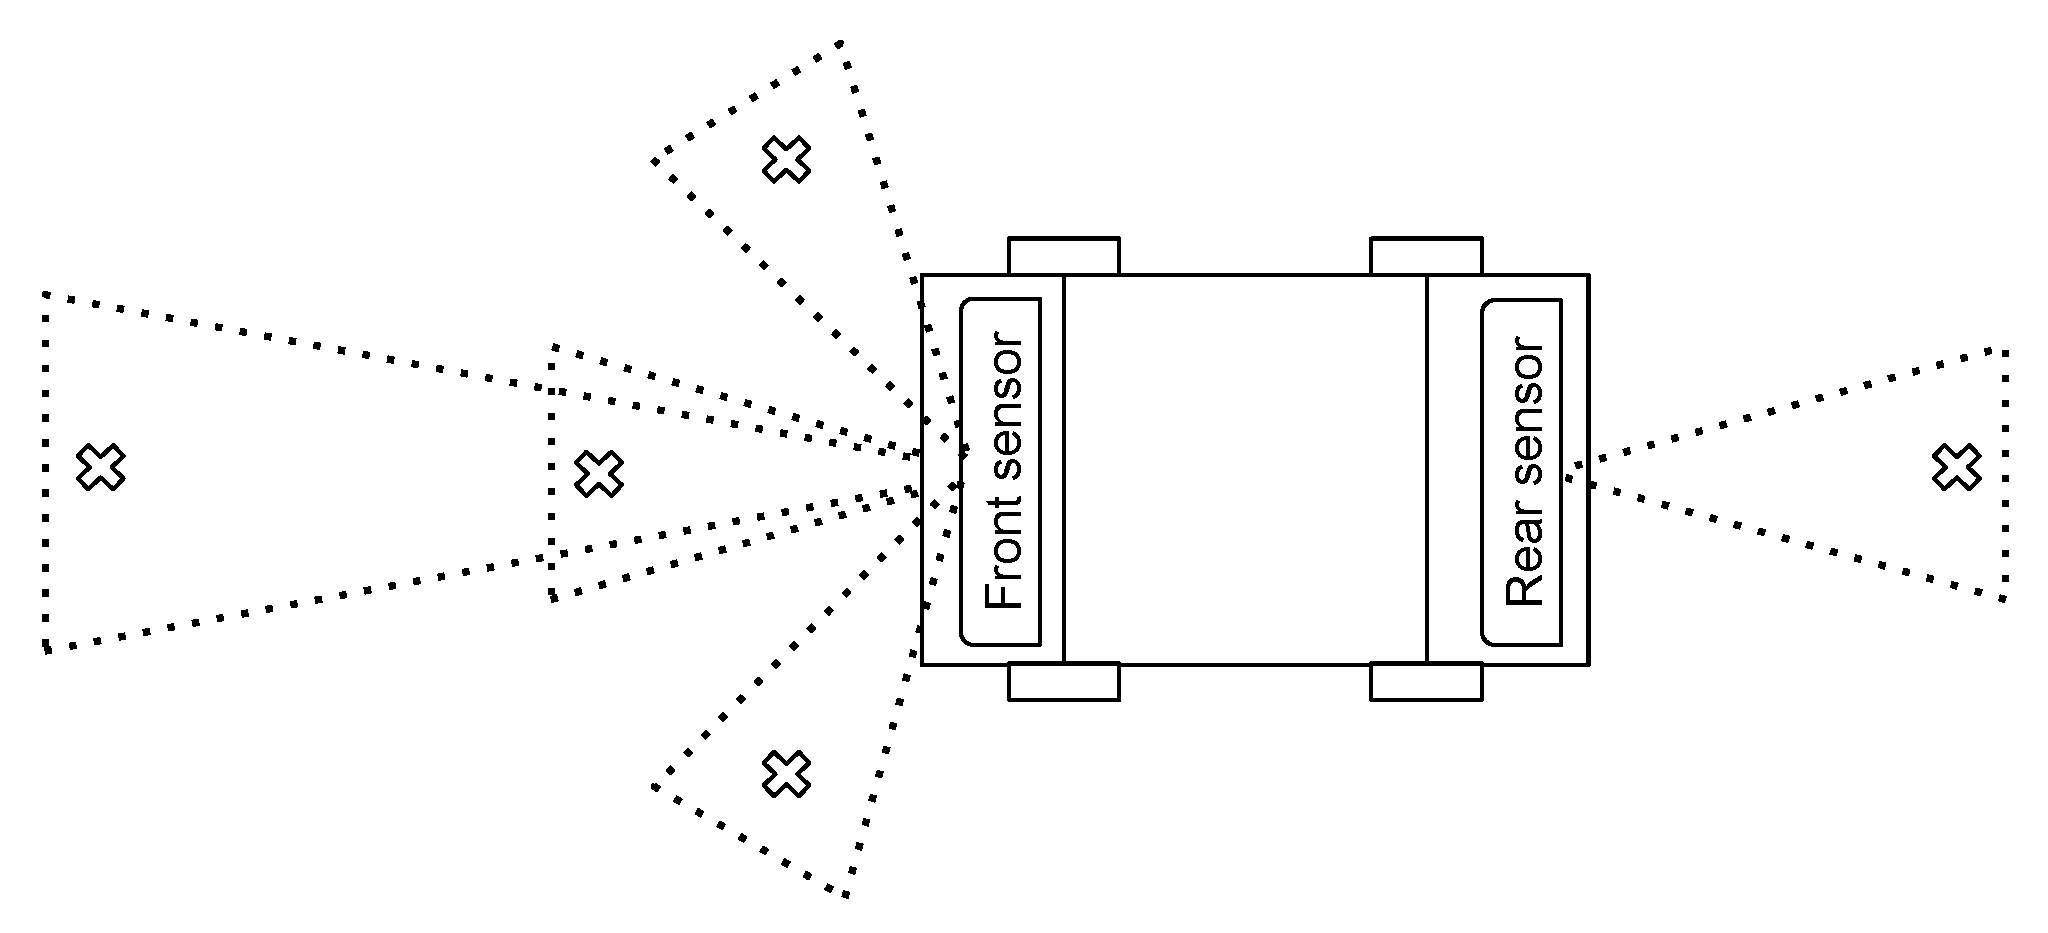
\includegraphics[width=\linewidth]{fig/AV.pdf}
		\caption{Sensor diagram for the AV safety system. \label{fig:car}}
	\end{figure}
\end{frame}
\begin{frame} \frametitle{AV System Block Diagram}
	\begin{figure}[t]
		\centering
		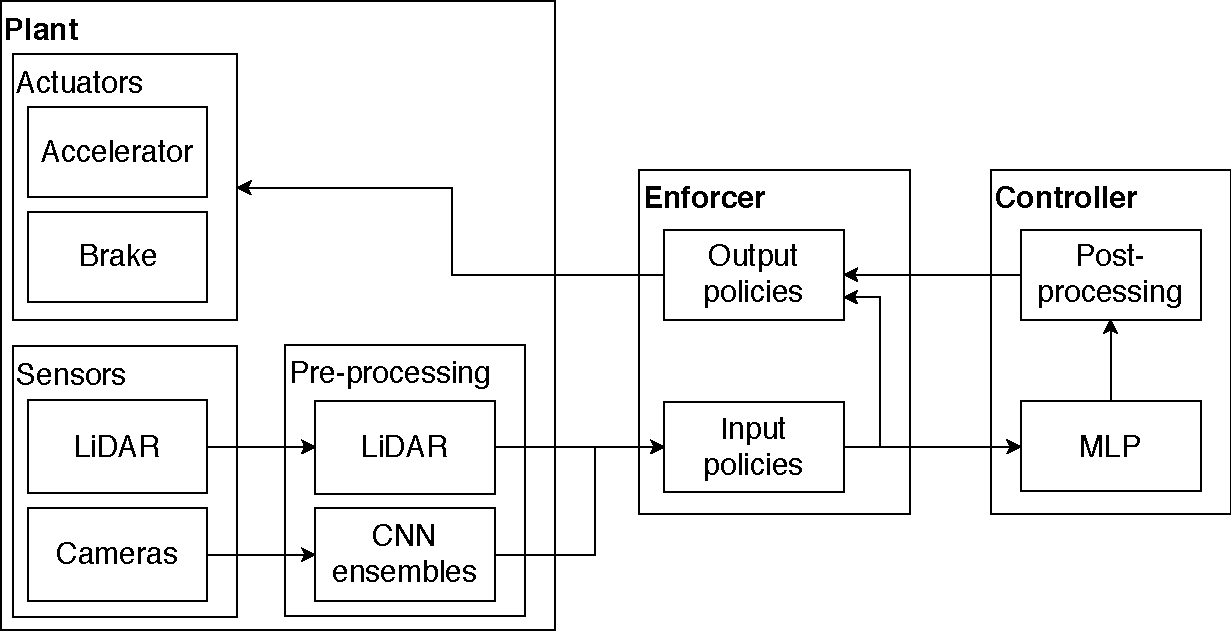
\includegraphics[width=\linewidth]{fig/AV-sys.pdf}
		\caption{Block diagram for the AV safety system. \label{fig:ubersys}}
	\end{figure}
\end{frame}

%\begin{frame} \frametitle{System Simulation: (AV)}
%	\begin{myitemize}
%		\item System too big and diverse to fully replicate.
%		\item Need partial simulation.
%		\item Ensemble must be trained off of a realistic data set
%		\begin{itemize}
%			\item VOC image dataset 2008. \footcite{voc2008}
%		\end{itemize}
%		\item LiDAR must be simulated
%		\begin{itemize}
%			\item KITTI autonomous vehicle dataset. \footcite{kitti}
%			\item Hours of data driving an autonomous vehicle.
%			\item LiDAR, cameras and GPS.
%		\end{itemize}
%	\end{myitemize}
%\end{frame}

\begin{frame} \frametitle{Runtime Enforcement}
	\begin{figure}[t]
		\centering
		\scalebox{1}{

\begin{tikzpicture}[>=stealth',shorten >=1pt,auto,node distance=4.5 cm, scale = 1, transform shape]

\tikzstyle{accept} = [draw=blue!75,fill=blue!20]
\tikzstyle{violate} = [draw=red!75,fill=red!20]

\node[initial,state, accepting, accept] (A) {$q_{drive}$};
\node[state, accepting, accept] (B) [right of=A] {$q_{brake}$};
\node[state, violate]         (C) [right of=B]  {$q_v$};

\path[->] 
		(A) edge [loop above]       node [above, xshift=-1em]  
		{
			\scriptsize$\let\scriptstyle\textstyle\substack{\overline{B_H}~\&~ \overline{(B_S~\&~P)}, \\ t := 0}$
		} (A)
		
		(A) edge [bend left=45]		node [above]  
		{
			\scriptsize$\let\scriptstyle\textstyle\substack{B_H~|~(B_S~\&~P), \\ t := 0}$
		} (B)
	
		(A) edge [bend right=70]	node [above]  
		{
			\scriptsize$\let\scriptstyle\textstyle\substack{\sum\textbackslash \Big((\overline{B_H}~\&~\overline{(B_S~\&~P)})~|\\~B_H~|~(B_S~\&~P)\Big)}$
		} (C)
	
		(B) edge [loop above]		node [above, xshift=2em]  
		{
			\scriptsize$\let\scriptstyle\textstyle\substack{(t < T_{lim}~|~B_H~|~B_S) \\~\&~\overline{A}}$
		} (B)
	
		(B) edge [left]				node [below]  
		{
			\scriptsize$\let\scriptstyle\textstyle\substack{\{t >= T_{lim}~\& \\ A~\&~\overline{B_H}~\&~\overline{(B_S~\&~P)}}$
		} (A)
		
		(B) edge [right]			node [below]  
		{
			\scriptsize$\let\scriptstyle\textstyle\substack{\sum\textbackslash \Big(t < T_{lim}~|~B_H~|~B_S|\\(t >= T_{lim}~\& \\ A~\&~\overline{B_H}~\&~\overline{B_S \& P})\Big)}$
		} (C)
	
		(C) edge [loop above]		node [above]  
		{
			\scriptsize$\sum$
		} (C)
		;

\end{tikzpicture}}
		\caption{Basic RTE state machine for the AV safety system \label{fig:rte}}
	\end{figure}
\end{frame}

%\begin{frame} \frametitle{Price / Demand example}
	%\centering
	%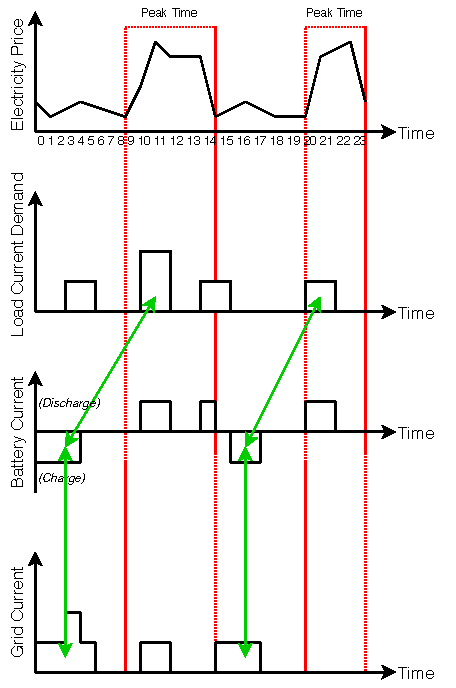
\includegraphics[scale=0.65]{fig/ess.pdf}
%\end{frame}

\section{Weekly progress}
\begin{frame}\frametitle{Autonomous Vehicle (AV) working example}
	\begin{block}{AV system}
		\begin{myitemize}
			\item Lots of TA marking...
			\item Training system with an increased number of epochs.
			\item Step from 10,000 to 100,000.
		\end{myitemize}
	\end{block}
\end{frame}

\begin{frame}\frametitle{Paper for IEEE journals}
	\begin{block}{TO-DO}
		\begin{myitemize}
			\item 
		\end{myitemize}
	\end{block}
\end{frame}

\section{Results}
\begin{frame}\frametitle{WCRT}
	\begin{itemize}
		\item WCRT tests were carried out on various, synchronous systems with SANNs.
		\item ABRO example utilizing SANNs shown below.
	\end{itemize}
	\begin{table}[H]
		\centering
		\caption{WCRT results for AI version of ABRO}
		\label{tbl:res-aibro}
		\begin{tabular}{|l|l|l|}
			\hline
			Approach         & WCRT (ms) & WCET (ms)\\ \hline
			Black-box        & 2.8  & 2.8  \\ 
			Layer by layer   & 1.9  & 7.6 \\ 
			Neuron by neuron & 1.8  & 7.2 \\ \hline
		\end{tabular}
	\end{table}
\end{frame}

\begin{frame}\frametitle{Meta neural networks}
	\begin{itemize}
		\item Using an meta neural network ensemble~\footcite{ensembleANN} of SANNs, it was shown that the combined accuracy of 3 SANNs was greater than the accuracy of any one SANN.
		\item Increase of up to 10\% from individual SANN accuracy.
		\item Retain synchronous semantics.
		\item Potential for WCRT analysis. 
	\end{itemize}
\end{frame}

\begin{frame} \frametitle{SNNs}
	\begin{table}[t]
		\centering
		\caption{Design and overhead of the policies used in the AV system}
		\label{table:policies}
		\begin{tabular}{|p{0.25\linewidth}|p{0.06\linewidth}|p{0.12\linewidth}|p{0.06\linewidth}|p{0.11\linewidth}|p{0.1\linewidth}|}
			\hline Policy & States & Transitions & Timed & Execution Time (us) & Overhead (\%) \\ \hline   
			%\multicolumn{6}{|p{0.70\linewidth}|}{\ac{AV}} \\ \hline
			$None$ 						&  &  &  & 736 & 0 \\
			$\varphi_{cnn}$ 			& 1 & 15 & No & 764 & 3.8 \\
			$\varphi_{drive}$ 			& 1 & 4 & No & 740 & 0.54 \\
			$\varphi_{car}$ 			& 1 & 7 & No & 774 & 5.1 \\
			$\varphi_{ped}$ 			& 2 & 56 & Yes & 767 & 4.2 \\
			$\varphi_{cnn} \wedge \varphi_{drive} \wedge \varphi_{car} \wedge \varphi_{ped}$ 	
			& 2 & 99 & Yes & 803 & 9.1 \\ \hline      
		\end{tabular}
	\end{table}
\end{frame}

\begin{frame} \frametitle{SNNs (cont.)}
	\begin{table}[h]
		\centering
		\caption{Results of the AV system with and without the enforced policies}
		\label{table:avenf1}
		\begin{tabular}{|p{0.15\linewidth}|p{0.15\linewidth}|p{0.15\linewidth}|p{0.15\linewidth}|p{0.15\linewidth}|}
			\hline Number of epochs trained & Percentage accidents & Average minutes to first accident & Average speed (km/h) & Percentage bad brakes \\ \hline
			\multicolumn{5}{|p{0.75\linewidth}|}{Not enforced} \\ \hline
			0 & 100	 & 3.21 & 98 & 19 \\
			1 & 100 & 3.3 & 93 & 19 \\
			10 & 100 & 3.8 & 81 & 57 \\
			100 & 100 & 5.35 & 59 & 24 \\
			1000 & 100 & 5.31 & 58 & 27 \\
			10000 & 48.5 & 73.9 & 18 & 63 \\ 
			80000 & 81.5 & 48 & 30.5 & ?? \\
			100000 & 93.9 & 35 & 31.5 & 65 \\ \hline                     
		\end{tabular}
	\end{table}
	\begin{myitemize}
		\item Less than 50\% accidents for the 10,000 epochs trained system
		\item 220 caused by collision from behind.
		\item 265 otherwise.
	\end{myitemize}
\end{frame}
\begin{frame} \frametitle{SNNs (cont.)}
	\begin{table}[h]
		\centering
		\caption{Results of the AV system with and without the enforced policies}
		\label{table:avenf2}
		\begin{tabular}{|p{0.15\linewidth}|p{0.15\linewidth}|p{0.15\linewidth}|p{0.15\linewidth}|p{0.15\linewidth}|}
			\hline Number of epochs trained & Percentage accidents & Average minutes to first accident & Average speed (km/h) & Percentage bad brakes \\ \hline
			\multicolumn{5}{|p{0.75\linewidth}|}{Enforced} \\ \hline
			0 & 75.7 & 756 & 45 & 0.7 \\
			1 & 70.2 & 828 & 47 & 4.2 \\
			10 & 88.5 & 589 & 37 & 20 \\
			100 & 79.5 & 726 & 41 & 17 \\
			1000 & 80.5 & 710 & 40 & 18 \\
			10000 & 63.6 & 910 & 30 & 27 \\ \hline                    
		\end{tabular}
	\end{table}
\end{frame}

\begin{frame} \frametitle{SNNs (cont.)}
	\begin{figure}[t]
		\centering
		\scalebox{1}{\begin{tikzpicture}
	\begin{loglogaxis}[
	xlabel={Number of epochs trained},
	ylabel={Time to first incident (/100)},
	x=0.8cm,
	y=1.2cm, 
	legend style={at={(0.1,0.55)},anchor=west}]
	
	\addplot[color=blue,mark=*] coordinates {
		(0,3.24)
		(1,3.29)
		(10,3.78)
		(100,5.53)
		(1000,5.74)
		(10000,27.41)
	};

	\addplot[color=red,mark=x] coordinates {
		(0,93.2)
		(1,94.5)
		(10,91.91)
		(100,94.5)
		(1000,94.2)
		(10000,96.69)
	};

	\legend{Policies not enforced, Policies enforced}
	\end{loglogaxis}%
\end{tikzpicture}%}
		\caption{Line graph showing the performance of the enforced system compared to the un-enforced system \label{fig:avgraph}}
	\end{figure}
\end{frame}

\section{Conclusion}
\begin{frame}\frametitle{Conclusion}
	\begin{itemize}
		\item 
	\end{itemize}
\end{frame}

\begin{frame}
	\printbibliography
\end{frame}

%\begin{frame} \frametitle{References}
%	\vspace{-16pt}
%	\begin{block}{}
%		\fontsize{5}{0}
		%\bibliographystyle{ieeetr}
%		\bibliography{../_paper/main} 
%	\end{block}
%\end{frame}

\appendix

\end{document}